\chapter{Tecnologie Utilizzate(template di prova - ANCORA DA SCRIVERE)}

\begin{figure}[h!]
	\centering
	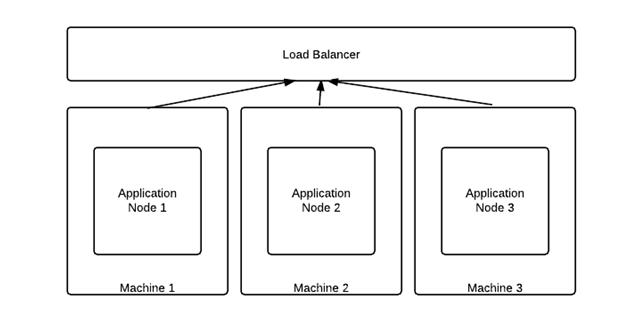
\includegraphics[width=\textwidth,keepaspectratio=true]{capitoli/imgs/LoadBalancer.png}
	\caption{Una schematizzazione della distribuzione del carico in una architettura Cloud}
\end{figure}


  \section{Linguaggi di programmazione}
    \begin{itemize}
     \item PHP 5.4.7 \\
     \href{http://www.php.net/}{http://www.php.net/};
     \item Javascript \\
     \href{http://www.w3.org/standards/webdesign/script}{http://www.w3.org/standards/webdesign/script};
    \end{itemize}
   \section{Linguaggi di Markup e Stile}
    \begin{itemize}
     \item HTML4/HTML5;
     \item CSS/CSS3;
    \end{itemize}
   \section{Framework}
    \begin{itemize}
     \item Smarty Template Engine \\
	\href{http://www.smarty.net/}{http://www.smarty.net/};
     \item JQuery\\
	\href{http://jquery.com/}{http://jquery.com/};
     \item JQueryUI\\
	\href{http://jqueryui.com/}{http://jqueryui.com/};
     \item beContent\\
	\href{http://www.becontent.org/}{http://www.becontent.org/};
    \end{itemize}
   \section{Ambiente di Sviluppo}
    \subsection{Eclipse}
      Per Eclipse sono state utilizzate due versioni differenti, la 4.2.2 in ambiente Windows e la 3.8.0 in ambiente Ubuntu/Linux \\
      \href{http://www.eclipse.org/}{http://www.eclipse.org/} \\
      Inoltre è stato utilizzato il pacchetto
      \begin{itemize}
       \item PHP Development Tools 3.1.1 \\
       \href{http://projects.eclipse.org/projects/tools.pdt}{http://projects.eclipse.org/projects/tools.pdt};
       
      \end{itemize}
    \subsection{Piattaforma Web}
      \subsubsection{XAMPP}
      \href{http://www.apachefriends.org}{http://www.apachefriends.org}
      \begin{itemize}
       \item Apache Web Server ver. 2.4.3 \\
	  \href{http://httpd.apache.org/}{http://httpd.apache.org/};
       \item MySql Database Management System ver. 5.5.27 \\
	  \href{http://dev.mysql.com/}{http://dev.mysql.com/};
      \end{itemize}
    \subsection{Browser Testing}
      \subsubsection{Mozilla Firefox}
	\begin{itemize}
	 \item Firebug ver 1.11.2 \\
	  \href{http://getfirebug.com/}{http://getfirebug.com/}
	    \begin{itemize}
	     \item Plug-In Validator ver. 0.0.6 \\
	      \href{https://addons.mozilla.org/it/firefox/addon/validator/}{https://addons.mozilla.org/it/firefox/addon/validator/};
	     \item Plug-In Google Page Speed ver. 2.0.2.3 \\
	      \href{https://developers.google.com/speed/pagespeed/?hl=it-IT}{https://developers.google.com/speed/pagespeed/?hl=it-IT};
	    \end{itemize}
	\end{itemize}
      \subsubsection{Google Chrome}
	\begin{itemize}
	 \item Strumenti per gli sviluppatori integrati 
	\end{itemize}
      \subsubsection{Responsive Testing}
	\begin{itemize}
	 \item Viewport Resizer- Responsive Design Bookmarklet \\
	 \href{http://lab.maltewassermann.com/viewport-resizer/}{http://lab.maltewassermann.com/viewport-resizer/} ;
	\end{itemize}



